% Chapter 4 - Player Study - Success factors

\chapter{Success Factors}
\label{chapter:player-study-success-factors}
\lhead{Chapter \ref{chapter:player-study-success-factors}. \emph{Player Study - Success Factors}}

This chapter examines the survey results in the context of determining the success factors of the game. The questions in Table \ref{tbl:rg1-survey-questions} and their answers are the main focus of this chapter, but relevant answers to other questions are also included.

\section{Results about Initial Interest}
\label{sec:success-factors-initial-interest-results}

To answer research question \ref{RQ1.1}, subjects were asked \emph{"Which of the following factors influenced your decision to start playing Pokémon GO?"}. Table \ref{tbl:initial-interest-options} shows the options that were supplied, as well as the number of respondents for each alternative. Subjects could choose more than one option, and the \emph{Other} choice allowed the respondent to describe other reasons.

\begin{table}[h]
	\caption{\emph{Which of the following factors influenced your decision to start playing Pokémon GO?} options and responses}
	\centering
	\label{tbl:initial-interest-options}
	\begin{tabular}{|l|c|c|}
		\hline
		\textbf{Option} & \textbf{Respondents} & \textbf{\% of total}\\
		\hline\hline
		Nostalgia or previous experience & 1507 & 70\\\hline
		Social media or internet forums & 764 & 35\\\hline
		Recommendations from friends/family & 738 & 34\\\hline
		Media coverage & 315 & 15\\\hline
		Official trailers/promotion & 308 & 14\\\hline
		The opportunity to get discounts or benefits & 9 & 0.5\\ because of Pokémon Go-related promotions && \\\hline
		Other & 165 & 8\\\hline
	\end{tabular}
\end{table}

The answers given for the \emph{Other} option were categorized, and Table \ref{tbl:initial-interest-other-categories} shows the categories with multiple answers, with the remaining responses grouped together as \emph{Miscellaneous}.

\begin{table}[h]
	\caption{\emph{Which of the following factors influenced your decision to start playing Pokémon GO?} Other categories}
	\centering
	\label{tbl:initial-interest-other-categories}
	\begin{tabular}{|l|c|c|}
		\hline
		\textbf{Category} & \textbf{Respondents} & \textbf{\% of Other}\\
		\hline\hline
		Pokémon & 43 & 26 \%\\\hline
		Exercise & 29 & 18 \%\\\hline
		Children/family & 26 & 16 \%\\\hline
		Ingress & 18 & 11 \%\\\hline
		Social & 7 & 4 \%\\\hline
		Technology & 6 & 4 \%\\\hline
		Fill outside time & 6 & 4 \%\\\hline
		Something to do & 5 & 3 \%\\\hline
		Real world & 5 & 3 \%\\\hline
		Trends & 4 & 2 \%\\\hline
		Gamer & 3 & 2 \%\\\hline
		Miscellaneous & 10 & 6 \%\\\hline
	\end{tabular}
\end{table}

The \emph{Pokémon} category are respondents who said they started playing simply because it was Pokémon. They consume any product related to the franchise, and would not let a Pokémon game go unplayed. These respondents are primarily around their twenties, and have to an extent grown up with Pokémon.

The \emph{Ingress} category are respondents who had previously played Ingress. Some active Ingress players were part of the Pokémon GO beta because of their participation, while others simply wanted to try another similar game. The \emph{Gamer} category are respondents who identify as gamers and picked up Pokémon GO because it was a new game, despite not having previous experience with either Pokémon or Ingress.

The \emph{Exercise} category are respondents who picked up the game as an exercise app, and wanted to use it as an excuse to walk more or a final push to get out and exercise, while the \emph{Fill outside time} are respondents who were already exercising or walking and wanted something to do during these activities.

The \emph{Children/family} category are respondents who either started playing because they wanted to spend time with their children or other family members who were already playing, or decided together with family members (significant others included) to start playing as a common activity. The \emph{Social} category are those who had similar goals with friends or who merely mentioned they started for the social aspect without specifying who they wished to be social with.

The \emph{Technology} category are respondents who were drawn to the game because of the technology used, be it augmented reality, GPS tracking or otherwise. The \emph{Real world} category are respondents who started playing because of the real world integration. They either wanted to find out what familiar locations had been turned into Pokéstops, or use the game to explore and find new and interesting locations. One subject in this category reported that they started playing because a sculpture they had made had been turned into a Pokéstop.

The \emph{Something to do} category are respondents who picked up the game just as something to do, either because they were bored at vacation or similar, or because they needed a distraction.

The \emph{Trends} category are respondents who started playing to take part in the cultural phenomenon and keep up with current trends.

\nice{Maybe add something about start time?}

\section{Analysis of Results about Initial Interest}
\label{sec:success-factors-initial-interest-analysis}

As expected, the Pokémon brand played a major role in spreading the game to such a vast number of players. 2164 respondents supplied a reason for downloading the game, and 1507 of them - almost 70 \% - listed \emph{Nostalgia or previous experience} as one of or the only reason they started playing. This reflects the large amount of respondents in their mid-to-late twenties as seen in Section \ref{sec:player-study-demographics}, as this is the age group who were children the last time Pokémon was a big deal, and people outside that age group are unlikely to feel nostalgia towards the phenomenon.

Releasing a Pokémon game that did not require any additional console (e.g. Nintendo DS), but could be played on the smartphone everyone was already carrying, was all but guaranteed to be a success. However, not all games can be Pokémon games, so what other things did Pokémon GO do right that we can use to create other successful games? A little over 30 \% of the respondents did not list nostalgia as a reason, and while some of them may have had memories of watching or playing Pokémon but for some reason or other did not pick this choice, there were certainly players who had no previous experience or connection with Pokémon.

The opportunity to get discounts or benefits because of Pokémon GO-related promotions did draw a few players, but with less than 0.5 \% of the respondents listing this as a reason, it seems negligible. Those who responded within the \emph{Pokémon} category can be grouped together with the nostalgia responders and should thus be ignored as well.

308 respondents, or just over 14 \%, said they were affected by official trailers or promotional material. This shows that the advertisements shown at Super Bowl 50 and available on Youtube were helpful in creating interest in the game. While 14 \% is a relatively small portion compared to the numbers for the other responses, the more casual players who were not reached by the survey (see more in Section \ref{sec:problems-with-survey}) may have had a larger portion of players who were intrigued by the Super Bowl ad but who did not have much previous experience with Pokémon.

\begin{figure}[h]
	\centering
	\caption{\todo{Screens from the ad shown at Super Bowl 50}}
\end{figure}

During the first few weeks following the release of the game, there was quite extensive coverage of the game in media all over the world. A little under 15 \% of respondents said that this media coverage affected their decision to start playing Pokémon GO, meaning it was slightly more effective than the official promotional material at building the player base, despite not an insignificant number of the articles posted were negative in their view \todo{(add some citations for negative articles)}. However, the media would not have covered the phenomenon to such a degree had there not already been a huge player base. But if one can succeed in spreading the game to a large enough number of players such that the media starts covering the game, it is not unlikely that one can achieve a similar growth of an additional 15 \% players. Those who responded within the \emph{Trends} category can also be included in this group.

A combined 69 \% of respondents said they started playing because of either recommendations from friends or family or from reading about the game on social media or internet forums. Similar to the \emph{Media coverage} group, these groups required someone else to pick up the game before them, but a huge following is not required for this to have an effect, unlike what is necessary for media coverage to kick in. Thus it could seem that if one can successfully spread ones game to an initial group of players and the game is appealing enough, it can easily spread naturally via them.

Veteran Ingress players were part of this initial group for Pokémon GO, and almost 11 \% of those who listed other reasons were previous Ingress players who either had been granted beta access to Pokémon GO or started playing it because they were previously familiar with the games from the developer. This also indicates that if a developer already has a successful game (even if somewhat niche, like Ingress), it is possible to adjust some parts of the game and release a new one and gain an initial player base from those familiar with your previous games. This is what game developers have been doing for years, and is also in line with \todo{Kiefer et al. (insert citation, "Systematically Exploring Design Space ...)}.

The \emph{Children/family} and \emph{Social} categories are partly related to the idea of creating an initial player base and letting it grow through sharing, but they also highlight the importance of the social aspect of the game. One area where Pokémon GO succeeded is making the game very social, and it becomes more fun to play together with others, as shown by 20 \% of the \emph{Other} responses placing in these categories. Players enjoyed going out to play with their friends and family, having a purpose and something to do while socializing. More on this in Chapter \ref{chapter:player-study-mental}. \todo{Add a note and citation for Coulton et al. (Harnessing Player Creativity ...) perhaps?}

The use of augmented reality technology and anchoring to the real world using GPS positioning also succeeded in attracting some number of players. About 7 \% of responses for the \emph{Other} option gave these areas as one of or the sole reason for playing. There still are not a large number of games using these technologies, and being one of the few that do allowed Pokémon GO to grab a market share by filling a hole. Some examples of other games with relative success in these areas were mentioned in Section \ref{sec:prestudy-ar-location-pervasive-games}, but there should still be room for more games in this category, and new, successful games could be created by changing some parameters of the Pokémon GO formula, as described in \todo{Kiefer et al.}

Another category related to real world integration is \emph{Fill outside time}. The respondents in this category take advantage of the location-based aspect of the game, where the game progresses simply by moving around. They were looking for an activity to fill the time they were already spending outside, either walking somewhere (e.g. to work, public transit etc.) or exercising, and a game that does not require their constant attention and actually progresses based on the activity they were already performing is a better fit than most other mobile games.

Even though Pokémon GO is not marketed as an exercise app, over 17 \% of respondents who chose the \emph{Other} option said they started playing the game with that exact purpose. The location-based gameplay serves as motivation to get up and out and to move around. With overweight being an increasing problem and sedentary lifestyles becoming increasingly common, we are frequently reminded by health institutions of the importance of physical activity. While most are aware that it is important to be physically active, many struggle with motivation. Not only being able to combine exercise with something fun, but the game actually requiring players to move around to progress makes Pokémon GO the perfect motivation for many players. Other games have also used a similar recipe to success before, as discussed in Section \ref{sec:prestudy-ar-location-pervasive-games}.

The \emph{Something to do} and \emph{Gamer} categories can also be more or less ignored, because it is difficult to say what will attract these players to your game over another one. The \emph{Gamer}s are likely to pick up any game they stumble upon, and the quality of the game will determine whether or not they will stick with the game. The respondents in the \emph{Something to do} category will similarly start any activity in an attempt to find something that can keep their attention. The best one can do to capture these players is to simply get the game as much exposure as possible to increase the odds of being the first activity or game they happen upon, and make sure the game is good enough to keep their attention. In the \emph{Miscellaneous} category are respondents whose reasons have too small of a sample size to draw any conclusions from.


\section{Results for Most Used Features}
\label{sec:success-factors-features}

To answer Research Question \ref{RQ1.2}, players were asked which of a selection of game features they used. The 2193 answers to this question are given in Table \ref{tbl:pokemon-go-features-used}.

\begin{table}[h]
	\centering
	\caption{\emph{Which of the following game features do you use?} responses}
	\label{tbl:pokemon-go-features-used}
	\begin{tabular}{|c|c|c|c|c|c|}
		\hline
		\textbf{Incubators} & \textbf{Gym battles} & \textbf{Lures} & \textbf{Incense} & \textbf{Shop} & \textbf{AR mode}\\
		\hline\hline
		2126	& 1729	& 1597	& 1427	& 1087	& 343\\
		97\%	& 79\%	& 73\%	& 65\%	& 50\%	& 16\%\\\hline
	\end{tabular}
\end{table}

\section{Analysis of Results for Most Used Features}
From Table \ref{tbl:pokemon-go-features-used}, we see that incubators were the most used feature of Pokémon GO (besides the obvious catching of Pokémon), with a massive 97 \% of respondents using this feature. With basis in the comments and answers across multiple questions, it seems likely that there are two major reasons for this popularity. The first half of it is the excitement and expectations the players experience because they don't know the contents of the egg. You never know exactly what you're going to get, and some eggs are known to contain rare and powerful Pokémon such as \emph{Snorlax} and \emph{Lapras}, which makes hatching eggs very desirable. The second half is that incubating eggs gives players something to do even if there is nothing else interesting in the immediate vicinity, or if the players are unable to pay attention to the game, for example while running.

Gym battles are the second most used feature. This seems natural, as they are currently the only points of interaction with other players within the game, and the only area of the game where players are able to deploy any sort of strategy, which for many is an important factor of playing games. As discussed in Section \ref{sec:quitting-reasons-the-grind}, gyms also provide the only goals in the game besides catching all the different Pokémon. Conquering gyms also provides rewards in the form of coins, which can be used to purchase things in the shop such as additional Pokéballs or incubators.

The third most popular feature were lures, used by 73 \% of the respondents. Lures, as discussed in Section \ref{sec:pokemon-go-in-depth}, are items used to attract Pokémon to specific Pokéstops. The Pokémon they attract can sometimes be rare Pokémon that do not frequently spawn in the area, making them attractive for players who are looking to catch more and rarer Pokémon. The lures also attract nearby players with the same goals. It was therefore not uncommon to see clusters of Pokéstops have lures on all Pokéstops, as groups of players would gather in these places to fill their Pokédexes and just hang out with old and new friends, making lures a very social item.

Incense was slightly less popular than lures, with 65 \% usage. Where the Pokémon attracted by lures are visible for all players, Pokémon attracted by incense are personal to the incense user. This makes it less attractive for use in groups, as players cannot split the costs of incense the same way they can with lures by rotating who places a lure. Incense does however allow players without access to Pokéstops to attract additional and rarer Pokémon, and in areas that do not naturally spawn Pokémon at all, lures are able to attract any Pokémon, making it popular in these areas.

The shop is especially important for players who do not have access to many Pokéstops, as they can often run out of Pokéballs. It is also the only way to get additional lures, incense, incubators and lucky eggs besides those awarded every ten levels. Therefore it is natural that it is relatively popular, considering the popularity of the features mentioned above. While it is used by 50 \% of the respondents, however, it is important to note that the coins required to purchase items in the shop can also be earned by capturing gyms, so it is likely that less than 50 \% actually spent money on the game. In the follow-up survey, 82 \% said they had spent real money in the store, with a median expenditure of roughly 770 NOK (or 90 USD), ranging from 55 NOK (around 6 USD) to 12000 NOK (around 1400 USD). There were only 11 respondents for these questions in the follow-up survey, however, so the significance of these numbers is unfortunately very low. These players spent coins primarily on incubators, secondarily on lucky eggs and storage space, and the rest on lures, incense and Pokéballs. Two of the low spenders spent coins only on Pokéballs.

Perhaps the most important number to note is the low usage of the \emph{AR Mode} feature. Only 16 \% of respondents used the AR mode, despite augmented reality being one of the important features in the promotional material and one several users listed as a reason to start playing in the first place. It is however not so surprising that players were reluctant to use it, as it sometimes made it more difficult to catch Pokémon because one would have to remain more or less stationary and point the phone towards the same location for the entirety of the catch while it was on. It also caused additional battery drain by using the camera, which was already a problem without AR mode, as discussed further in Section \ref{sec:quitting-reasons-technical-requirements}. One would think that these problems and the low usage indicated that it was mostly only used by low level, new players, but the usage was in reality distributed evenly with player levels ranging from 7 to 38.

We see that the items that increased the amount of Pokémon the players get access to, that is the incubators, lures and incense, were all very popular. By purchasing these items in the store, the player can increase their pace of play by encountering more Pokémon and more quickly gaining access to stronger Pokémon, and are not unlike the items that can be purchased in other mobile games. They provide an advantage to those players who purchase them, but one that can also be gained by spending an appropriately higher amount of time in the game. That there are no items available for purchase that give advantages that cannot be otherwise be gained by putting extra effort into playing is an important trait of the game that multiple players mentioned in comments and the follow-up survey as reasons that would make them quit the game.

That the augmented reality part of the game was so little used means that there is some room for improvement here. It adds a little bit of immersion to the game, and allows for funny or interesting photos to be taken, but beyond that there is little reason to use it at all. John Hanke, the CEO of Niantic, mentioned in an interview with Business Insider \todo{[cite interview]} that they were planning on extending the feature in the future. Nothing has come of it yet, but it seems important if they want to be able to compete in this section of the market.

\section{Results for Dwindling Interest}
Despite launching as a soaring success, the Pokémon GO bubble also burst relatively quickly. Player numbers started dwindling near the end of July as seen in Figure \ref{fig:player-numbers}, and by mid-August it had lost around 80 \% \todo{(check the number and get citation here)} of its active player base. This section and the following attempts to answer research question \ref{RQ1.5} and determine why Pokémon GO all but faded away so quickly.

\begin{figure}[h]
	\centering
	\caption{\todo{Insert figure of global player numbers}}
	\label{fig:player-numbers}
\end{figure}

Table \ref{tbl:still-playing} shows the distribution of responses for the question \emph{"Are you still playing?"}. Not surprisingly, less than 3 \% of the responses said they had already quit playing, as those who have quit are for the most part no longer following Pokémon GO groups or forums even if they previously were. What is more interesting is that over 40 \% of respondents said they had reduced the amount of time they play compared to their peak. While we do not know how much they reduced their play time, we do know that they were playing less, and there had to be some reason for it.

\begin{table}[h]
	\centering
	\caption{\emph{Are you still playing?} survey question responses}
	\label{tbl:still-playing}
	\begin{tabular}{|c|c|l|}
		\hline
		\textbf{No} & \textbf{Yes} & \textbf{Yes, but less frequently than during my peak}\\
		\hline\hline
		65 & 1245 & 884\\
		3\% & 57\% & 40\%\\\hline
	\end{tabular}
\end{table}

A total of 610 respondents gave one or more reasons for either quitting the game or reducing the amount of time they spend in the game compared to their peak. These answers were categorized into one or more categories depending on the given reason. Table \ref{tbl:reasons-for-quitting} shows these categories, along with the number of respondents who gave a reason that was placed in that category, and the portion of the total number of respondents who gave reasons. It should be noted that the input for this question was free text. Because some of the categories are closely related, and because the interpretation of some answers may have been slightly wrong, some respondents may have been placed in one category when they should have been in another similar one instead.

\begin{table}[h]
	\centering
	\caption{Reasons for quitting or reducing play time of Pokémon GO}
	\label{tbl:reasons-for-quitting}
	\begin{tabular}{|l|c|c|}
		\hline
		\textbf{Category} & \textbf{Respondents} & \textbf{\% of total}\\
		\hline\hline
		Reduced free time & 253 & 41 \%\\\hline
		Non-urban & 77 & 13 \%\\\hline
		Social aspect & 51 & 8 \%\\\hline
		Too repetitive & 45 & 7 \%\\\hline
		Lack of features/content & 43 & 7 \%\\\hline
		Difficulty of progression & 41 & 7 \%\\\hline
		Goal completion & 40 & 7 \%\\\hline
		Lack of variation & 40 & 7 \%\\\hline
		Hype died down & 39 & 6 \%\\\hline
		Removal of tracker & 38 & 6 \%\\\hline
		Climate/weather & 28 & 5 \%\\\hline
		Community management & 26 & 4 \%\\\hline
		Technical requirements & 21 & 3 \%\\\hline
		Technical issues & 13 & 2 \%\\\hline
		Cheaters/catching up & 13 & 2 \%\\\hline
		Burnout & 9 & 1 \%\\\hline
		Lack of purpose/endgame & 9 & 1 \%\\\hline
		Lack of incentives & 8 & 1 \%\\\hline
		Too all-encompassing & 7 & 1 \%\\\hline
	\end{tabular}
\end{table}

The largest category by far was \emph{Reduced free time}. This category consists of respondents who had either quit playing or reduced the amount of time they play because of reduced free time. The cause of the reduced free time was in most cases related to returning to work or school/studies. The \emph{Climate/weather} category is related, being additional players who decided to play less as summer faded away, but for climate and weather reasons rather than (or in addition to) having less time available.

The \emph{Non-urban} category are respondents who live outside urban centers, either in suburban or rural areas. These areas are not as suited for Pokémon GO playing as urban areas, and is sometimes referred to as \emph{the rural problem}. More on this issue in Section \ref{sec:the-rural-problem}.

The \emph{Social aspect} category are those who quit or reduced play time because the game fell in popularity with others and they did not have as many other people to play with. Somewhat related is the \emph{Hype died down} category, which consists of respondents who got bored with the game after the novelty wore off and the game was no longer \emph{"hyped"} as much.

The \emph{Too repetitive} category focuses on the repetitiveness of the game. These respondents felt like they were doing the same thing over and over and felt their enjoyment of the game (e.g. catching the same Pokémon, evolving them and then transferring them) lessen because of this. The \emph{Lack of variation} category is closely related, consisting of players who were tired of mostly only running into the same Pokémon everywhere. This is also somewhat related to \emph{the rural problem}, as the variety of Pokémon becomes much smaller once you leave the urban areas.

The \emph{Lack of features/content} category is again closely related to the previously mentioned \emph{Too repetitive} category. These players got bored of the game because of the limited number of things one can do within the game itself. You are limited to relatively few activities, as described in Section \ref{sec:pokemon-go-in-depth}, and this was simply not enough to keep the interest of these players in the long run. The \emph{Lack of purpose/endgame} category is relevant here, consisting of players who struggled to find a purpose with the game. There was no clear goal or endgame, and thus nothing for these players to works towards.

The \emph{Difficulty of progression} category respondents were frustrated with how long it takes to make any progress after having played for a while. The related \emph{Lack of incentives} category focuses on the lack of incentives to progress or even play the game.

The \emph{Goal completion} category are players who had certain goals when they started playing. As they reached these goals, they no longer felt any reason to play, or at least no longer played as actively. For most of these players, the goal was to catch one of each Pokémon (or at least those available to them in their region). For others, additional goals were to reach certain player levels in the game.

The \emph{Removal of tracker} category consists of players who were unhappy about the removal of the in-game tool for tracking Pokémon. For the first few weeks after the initial release of the game, players could track Pokémon in the area by using a tool that was available within the game itself. The \emph{tracker} showed from one to three footprints next to an image of the Pokémon, indicating its distance from your current location. As the player got closer, the number of footsteps would decrease. However, around July 18th, this tracker stopped working, never showing less than three footsteps. For some time it was believed that this was caused by a bug, but within two weeks, the footsteps feature was removed entirely. The players in this category were not happy about this, and either reduced play time because of it, or quit playing entirely.

Many players were not happy about the way this issue was handled. The feature was "broken" for a long time without any news from the developers about it, leaving players not knowing whether it was a bug that would be fixed or if it was intentional. For a long time there was a general lack of communication from Niantic regarding the game at all, and the \emph{Community management} category consists of players who were frustrated about this to the point where they no longer wished to play as actively, or in some cases at all.

The \emph{Technical requirements} category are respondents who decided that the technical requirements of the application were too much for them to be willing to play, or who actually were unable to play because of them. One of the requirements that many struggled with was the huge battery drain playing the game caused. The game required the screen to be on, and was constantly using GPS and mobile data, resulting in a battery drain that caused most users to have to charge their phone several times a day. This lead to a massive spike in power bank sales, but for some it was simply not feasible or acceptable to charge multiple times during the day. For others, the issue was with the use of mobile data, having too a too limited amount of data available to let the game use it all. A third, major technical requirement that completely lost a portion of players was the requirement for the device to not be rooted. This was a change made in early September in an attempt to stop cheaters, that also ended up rendering many legitimate users who had rooted their Android devices for one reason or other unable to play the game. Many of these users were infuriated with Niantic, also responding within the \emph{Community management} category.

The respondents in the \emph{Cheaters/catching up} category are players who wished to compete in gyms, but were unable to because they were too far behind. While some of these respondents were players who had been forced to take a break or were late to the party and fell behind because of that, the majority of this category are people frustrated with cheaters. Pokémon GO has struggled with players cheating through various means, such as creating bots that can play constantly, and \emph{spoofing} their GPS-location so they can be anywhere in the world at any moment. This resulted in very high level rare Pokémon filling gyms around the world, making it difficult for legitimate players to compete.

In the first few weeks after release the game was suffering from technical issues of varying degree of severity. The game was full of bugs, some worse than others, but the major problem was the servers. They were not proportioned for the incredible amount of players, and during peak hours (the middle of the day in America) you were lucky if you were able to log into the game. If you were unlucky enough to encounter one of the bugs that required you to restart the game, you were all but forced to stop playing for the rest of the day. This annoyed quite a few players, and for some of them it was not worth it trying to play. These players are represented in the \emph{Technical issues} category.

The last categories are the \emph{Too all-encompassing} and \emph{Burnout} categories. The \emph{Burnout} category are players who went all-out and played too much and got burnt out and tired of the game, while the \emph{Too all-encompassing} players could no longer deal with everything around them being about Pokémon. They were either unable to focus on anything other than Pokémon themselves, or everyone around them talked about nothing else, and it became too much for them.

Other answers that had less than 1 \% representation were not included in the table. Some examples are players who were unsatisfied with the combat system and the difference from the Nintendo device based games, players who disliked the lack of variety in the Pokémon you would encounter in gyms, or were unhappy that they were unable to hold a gym even if they placed their strongest Pokémon in it. Some did not approve of the decision to make some Pokémon region-specific, while others found the game unrealistic because even the weakest of Pokémon were sometimes quite difficult to catch, and some did not like that the Pokémon they could catch in the wild almost always were much weaker than those they would hatch from eggs. Some did not want to use the app because of security concerns, some gave up saying they were too lazy to play it, and some simply found the game to be boring.

\section{Analysis of Results for Dwindling Interest}
\label{sec:success-factors-quitting-analysis}

\todo{Short intro to this section}

\subsection{Reduced free time}
\label{sec:reduced-free-time}
We saw that the vast majority of players who had quit or reduced their play time had done so because they simply did not have enough spare time to play anymore. Releasing the game during summer when schools were out and adults were taking out their vacation allowed the game to build a much larger player base than if it had released during a busier time. While a lot of the players are not sticking around in the long run, it was still a successful strategy. As we saw from the number of players who were drawn to the game because of friends, family, social media and media coverage in Section \ref{sec:success-factors-initial-interest-results}, the important part was to get a large initial player base that would expand naturally. Even if some (or even most) of the players who started because they had time during summer stopped playing entirely after their vacation ended, many of the people they brought to the game may have stayed. At its peak, Pokémon GO was earning more money than all other mobile games combined \todo{[cite Forbes/Slice]}, and even after losing most of its player base it remains one of the most profitable mobile games available.

\subsection{Removal of tracker}
While less than 7 \% of respondents mentioned the removal of the tracker as a reason for quitting or playing less, it has been one of the most discussed topics in the Pokémon GO community since it happened. The tracker was not only very important to the playability of the game, but core to the concept and idea of being a Pokémon trainer. The players want to go out and be able to hunt for specific Pokémon to \emph{"catch 'em all"} and complete their \emph{Pokédex}, or to get certain strong Pokémon for battling with. With the removal of the tracker, the players were forced to walk around aimlessly, hoping to be fortunate enough to run into the Pokémon they wanted to find.

Shortly after the removal of the tracker, third-party map services started popping up online. These services let players choose an area they wished to search in, and the service would run API calls to the same API as the game itself to find what Pokémon were currently available in the area, and placed them on a map. For a large number of players these services became the new tracker, and they became more focused in their playing, going to specific locations because of the Pokémon they knew were present rather than because of the density of Pokéstops.

Some players viewed these maps as blatantly cheating, while others viewed them as a necessary evil. Others argued that they made the game more realistic, as if the Pokémon were real, there would indeed be data mapping where the different species could be found. Niantic were clear on their stance, however: the maps were cheating, and their creators were sent cease and desist letters \todo{[cite someone reporting this, e.g. Kotaku]}. The sites were taken down, and users were once more stuck without a functioning way of tracking Pokémon. This caused further outrage among players, and the player base was largely unhappy with the way Niantic were handling the community. The in-game tracker was still broken, without much word from the developers on their progress in getting it back.

The tracker has since been re-introduced in a new version: it still lists Pokémon that are nearby with no indicator of distance, but Pokémon that are near Pokéstops now list the closest stop and can even be shown on the in-game map. However, the whole tracker situation shows two major things that should be important to keep in mind when creating a popular game:

\begin{enumerate}
	\item Do not remove core functionality from the game after it has been released. If absolutely necessary:
	\item Make sure you have a handle on community management. If the game becomes popular, you will get support requests, and if they do not get answers, your players will be unhappy and eventually leave.
\end{enumerate}

\subsection{Social aspect}
\label{sec:success-factors-social}
The 8 \% of players who leave because the social aspect became worse are difficult to avoid, but they show the importance of the strong community and maintaining a good player base. One player went as far as saying \emph{"A vibrant competitive community is more important that the actual content of the game"}. The fact that players were able to compete but still play together and cooperate despite being on different teams was a nice feature appreciated by many players, and is discussed further in Section \ref{sec:mental-health-relationships}.

\subsection{Non-urban}
\label{sec:the-rural-problem}
Almost 13 \% of players ended up losing their enthusiasm for the game, and in some cases leaving entirely because the game for a long time was all but unplayable in rural areas, and strongly imbalanced towards urban areas. There are multiple sides to this issue, but it is clear that something should have been done differently, as we can see not only from it driving players away, but from the fact that Niantic later increased the spawns for rural areas.

The core of \emph{the rural issue} is that urban centers had a much higher density of Pokéstops, gyms and Pokémon spawns - everything needed to participate in the game - than non-urban areas such as suburbs or rural areas. As explained in Section \ref{sec:pokemon-go-in-depth}, this is because Pokéstops and gyms were based on points of interest reported by players, while Pokémon spawns (initially) were based on cell phone usage.

It makes sense that cities and urban centers have more Pokéstops and gyms, for multiple reasons. From a technical perspective, there are typically more points of interest in a more densely populated area, and these areas were more likely to have Ingress players who would report these \emph{POI}s to be registered. From an immersion perspective, it's also not hard to believe that more people would set up gyms or hotspots to help nearby trainers in cities where more trainers are likely to come by.

The immersion perspective is where distribution of Pokémon spawns fails, however. While it makes sense from a technical perspective to use mobile usage to place spawns because it avoids having many spawns that no one will ever see because they are in areas where no one travel, from an immersion perspective it does not make sense that wild Pokémon are more likely to converge in areas filled with humans as opposed to being out in nature. Rural areas had close to no spawns, and the few they had were mostly just of the common species \emph{Pidgey} (a pigeon-like bird Pokémon) and \emph{Rattata} (a purple rat Pokémon). These are Pokémon you would expect to find in a city, while rare Pokémon such as \emph{Charizard} and \emph{Dragonite} (large dragon Pokémon), \emph{Aerodactyl} and \emph{Kabutops} (living fossil Pokémon) and \emph{Onix} (an enormous stone snake Pokémon) are examples of Pokémon you would not expect to find on a busy pier or shopping street. There are plenty of the common Pidgey and Rattata in cities as well, but where almost every single spawn in rural areas are these Pokémon, the cities have plenty of other spawns as well, including rare and dangerous (from an in-universe perspective) Pokémon. Players in suburban areas are to a degree better off than the rural players, with slightly more spawns and a little higher variation in the species they encounter, but they too have nothing compared to the truly urban players.

\begin{figure}[h]
	\centering
	\caption{\todo{Rare Pokémon, perhaps in strange environments}}
\end{figure}

\begin{table}[h]
	\centering
	\caption{\emph{What type of area do you primarily play in?} answer distribution}
	\label{tbl:urban-level-distribution}
	\begin{tabular}{|c|c|c|}
		\hline
		\textbf{Urban} & \textbf{Suburban} & \textbf{Rural}\\
		\hline\hline
		1048	& 919	& 227\\
		48\%	& 42\%	& 10\\\hline
	\end{tabular}
\end{table}

Because a large part of the player base naturally would be located in cities, it was important from a community perspective to enable them to play the game, and removing all exciting spawns from cities therefore seems like an equally bad or worse alternative. However, since much of the player base also lives and plays outside of cities, they too should be able to play. Table \ref{tbl:urban-level-distribution} shows the distribution of survey respondents between the three environments. With the described system, urban players gained an unfair advantage, not only having better and frequent access to rare Pokémon, but also being able to stock up on consumables from Pokéstops where suburban and especially rural players were lucky to have more than one Pokéstop around from which they could gather Pokéballs. The result of these differences was that urban and suburban/rural players were essentially playing different games. Urban players who visited suburban or rural areas and players from the suburbs or rural areas who worked in and commuted to more urban areas brought this unfair advantage with them and were able to place strong Pokémon acquired in the city in the few gyms available in the outskirts. In December, Niantic added additional spawns to rural areas (as well as to parks), but it may have been too late. \todo{Add some citation, maybe screenshot of the official tweet}

\nice{Maybe mention Lapras event?}

\subsection{Cheaters and catching up}
\label{sec:cheaters-analysis}
Only a little over 2 \% of respondents listed cheaters and the difficulty of catching up and competing as a reason to quit. This is likely because most of the game can still be played in spite of cheaters and people who have been playing more than you. The only affected aspect of the game are gyms, as that is currently the only place where players interact with each other inside the game itself. However, in the area where it does matter, it is clear that cheaters are significant problem. While not all gyms are being targeted by these cheaters, in some popular areas players are finding it impossible to hold a gym for more than a few minutes, even in the middle of the night, as high level trainers suddenly show up in the game to claim the gym and fill it with powerful Pokémon, despite there being no one else around. Perhaps the best example of this problem is that within a few hours of the game's release in Brazil, many gyms were already filled with level 30 trainers and their nigh unbeatable Pokémon. For reference, the total amount of experience points needed to reach level 30 is 2 000 000 (two million), while catching a Pokémon nets 100 experience points, making the feat of one player reaching level 30 within less than a day of release impossible. With all nearby gyms full of these trainers, Brazilian players were not thrilled.

Niantic made multiple changes throughout the year in an attempt to make it more difficult for cheaters, in addition to banning known and suspected cheaters' accounts, but because letting a bot play for you requires minimal effort, they keep creating new accounts. For those who want to play the game competitively but are unwilling to cheat, better solutions are needed. \todo{Make some suggestions here, e.g. show time Pokémon was added to gym}

\subsection{The grind}
\label{sec:quitting-reasons-the-grind}
Over 7 \% of players who quit the game found the game to be too repetitive, while almost 7 \% were less motivated to play because of the difficulty of progression. These two categories combined make up the more than 14 \% who complained about the \emph{grind} \todo{(one sentence explaining what the grind is)} the game turned into. Starting at level 20, the number of experience points (\emph{XP}) needed to progress to the next level increases rapidly. Figure \ref{fig:experience-per-level} shows the required experience to reach each level along with the total accumulated experience so far for levels 18 and up.

\begin{figure}[h]
	\centering
	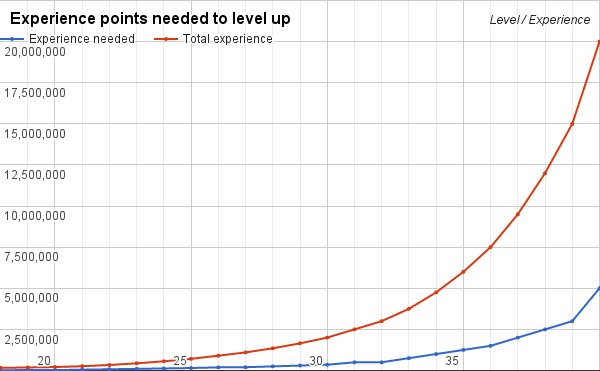
\includegraphics[width=\textwidth]{Figures/experience-per-level}
	\caption{Experience points needed to level up from level 18 to 40}
	\label{fig:experience-per-level}
\end{figure}

%\begin{table}[h]
%	\centering
%	\caption{Experience points (XP) needed to reach levels}
%	\label{tbl:experience-per-level}
%	\begin{tabular}{|r|l|l|}
%		\hline
%		\textbf{Level} & \textbf{XP needed} & \textbf{Total accumulated XP}\\\hline\hline
%		18 & 20 000 & 160 000\\\hline
%		19 & 25 000 & 185 000\\\hline
%		20 & 25 000 & 210 000\\\hline
%		21 & 50 000 & 260 000\\\hline
%		22 & 75 000 & 335 000\\\hline
%		23 & 100 000 & 435 000\\\hline
%		24 & 125 000 & 560 000\\\hline
%		25 & 150 000 & 710 000\\\hline
%		26 & 190 000 & 900 000\\\hline
%		27 & 200 000 & 1 100 000\\\hline
%		28 & 250 000 & 1 350 000\\\hline
%		29 & 300 000 & 1 650 000\\\hline
%		30 & 350 000 & 2 000 000\\\hline
%		31 & 500 000 & 2 500 000\\\hline
%		32 & 500 000 & 3 000 000\\\hline
%		33 & 750 000 & 3 750 000\\\hline
%		34 & 1 000 000 & 4 750 000\\\hline
%		35 & 1 250 000 & 6 000 000\\\hline
%		36 & 1 500 000 & 7 500 000\\\hline
%		37 & 2 000 000 & 9 500 000\\\hline
%		38 & 2 500 000 & 12 000 000\\\hline
%		39 & 3 000 000 & 15 000 000\\\hline
%		40 & 5 000 000 & 20 000 000\\\hline
%	\end{tabular}
%\end{table}

As we can see, the required experience to level up past 20 starts increasing much more rapidly than for the first 20 levels, where the total amount of experience needed to reach level 20 is 210 000, while level 30 requires a total of 2 000 000 (two million), and 40 requires 20 000 000 (twenty million). After level 30 the experience required to level up becomes too much for most players, and when the player reaches level 37 they are still not halfway to level 40.

Every caught Pokémon only yields 100 XP with no regard towards the difficulty of the catch or the strength of the Pokémon, while evolutions yield 500 XP, again disregarding the strength of the Pokémon or the amount of resources needed to perform the evolution. While bonuses for \emph{nice}, \emph{great} or \emph{excellent} throws, as well as a bonus for throwing a curved ball, can grant up to 110 additional XP per catch, the strategy that is widely regarded as the most efficient way to level up is mass evolution of common Pokémon such as Pidgey and Rattata. By activating a \emph{lucky egg}, a purchasable item that doubles XP earned for 30 minutes, and then performing around 90 evolutions, players are able to earn up to 90 000 XP in one "session". Unfortunately, at higher levels, this is more or less the only time any significant progress is made, which makes players less motivated to play more after reaching level 30. At this point, most have "completed" their Pokédex (more in Section \ref{sec:pokemon-availability-and-goal-completion}), and their entire play experience revolves around catching the same marginal selection of Pokémon (for most this is Pidgey, Weedle and Rattata), then evolving and transferring them once they have enough candy to perform around 90 evolutions.

Combine this monotonous experience with the lack of incentives (which around 1.31 \% reported as a reason to stop playing) and the game does not sound very appealing. At level 20, Pokémon hatched from eggs stop scaling with the player level (all Pokémon caught after level 20 are hatched as level 20). At level 30, wild Pokémon stop scaling further (you can never encounter wild Pokémon higher than trainer level 30). While every level awards some number of consumables (different types of Pokéballs, potions etc.), and every few levels unlocks a new type of item, the last type of item is unlocked at level 30. Every additional level the trainer gains allows powering up their Pokémon a little further, but beyond this there are no real incentives to level past 30.

There also seems to be no real purpose or endgame, which around 1.5 \% listed as a reason for quitting. As players catch new Pokémon and continually improve the ones they catch, there is no in-game goal to work towards \todo{(something about intrinsic and extrinsic motivation in chapter 2?)}. Currently, the only actual use for Pokémon is to battle at gyms. Capturing gyms lets you claim up to 100 in-game coins (10 per held gym at the time of the claim) once per 21 hours. These coins lets you upgrade your storage space or purchase consumables that either let you get more Pokémon or level up so you can have stronger Pokémon. If you are able to capture many gyms, people in your local community may start to recognize your name, but beyond that there is no recognition to be had, and there are no real life rewards.

Gym battles favor the attacker (see more on how gyms work in Section \ref{sec:pokemon-go-in-depth}), which makes it very difficult to hold gyms for any significant amount of time, and in popular areas the gyms often switch controllers multiple times per hour. Because of this there is little incentive to level up and improve your Pokémon.

In the original games and the animated TV series, gyms were locations held by certain esteemed trainers and the player had to defeat eight of these to collect \emph{badges}. Collecting all eight badges allowed the player entry into the \emph{Pokémon League}, a very difficult tournament where the winner was crowned Champion. Subsequent entrants into the league would have to battle the previous Champion at the end to try to become the next Champion. The League was very tough, and required very strong Pokémon to be able to defeat. Implementing something like this into the game would provide a goal for players to work towards, and a reason to keep progressing to higher levels. Other multiplayer games often have online leader boards where strong players are showcased. This is another way of giving players motivation to keep playing and become stronger trainers, and is something the Niantic CEO mentioned in an interview shortly after the release \todo{[cite Business Insider interview]} that they were planning on implementing, but has yet to be seen at the time of writing this.

It makes some sense to make it difficult to reach the highest level, not only to keep some difference between the dedicated players and the casual players, but also to make it prestigious and desirable to reach the goal - given that there are incentives to do so, as discussed above. However, the current solution of almost exponential growth in required XP seems somewhat absurd given the flat rates of XP rewards. While it is true that a large part of the game's business model is based on sales in the in-game shop, and requiring large amounts of experience to level promotes sale of the \emph{Lucky Egg} item which doubles experience  gained for 30 minutes, a player could level ten times to level 30 in the time it takes to reach level 40. Leveling to level 30 in a reasonable amount of time still requires active usage of Lucky Eggs, and if the higher levels were slightly less out of reach, more players might be inclined to purchase these Lucky Eggs and go all the way to the top. If the amount of experience needed to reach level 40 was halved to ten million, it would still be a considerable feat, but many more players would likely attempt to reach the goal.

One way to combat the feeling of grinding without changing the amount of experience needed to level is to change the reward systems. Currently, the reward for catching a Pokémon is 100 XP (plus the potential throw bonus), 3 candy of the appropriate type, and 100 stardust, regardless of whether the Pokémon has a combat power (CP) of 10 or 2 000 and whether you spent one regular Pokéball or eight Ultra Balls to catch it. In most games, harder feats yield higher rewards, so why can Pokémon GO not work this way? Unless the player has nigh unrestricted access to Pokéballs, there is little reason to waste many balls on trying to catch a stage 2 or 3 evolution when catching unevolved Pokémon is easier, yields the exact same rewards, and is actually better because they can be used to gain more XP through evolution.

Since evolution costs candy, it would make sense that catching an evolved Pokémon yields more candy of the appropriate type, perhaps along with some additional XP and stardust. Performing a third stage evolution costs more candy than a second stage evolution, so unless you are missing the Pokémon from your Pokédex or are going to use the evolved Pokémon to battle, there is never any reason to evolve past the second stage. If these evolutions yielded an appropriately scaled XP reward, perhaps along with some other reward (e.g. stardust), it's much more likely players would be willing to switch up their current routine. By providing bonuses for catching or evolving different Pokémon, even more variation could be introduced.

Games like \emph{Candy Crush Saga} can get away with less variation in game play because they are games typically played while doing something else, e.g. traveling, and often require the user to think strategically. Pokémon GO on the other hand requires active participation because you have to physically move for the game to progress. It also requires little to no strategic thinking. In the original games the player could battle wild Pokémon to weaken them, making catching them easier. Implementing this feature would make the game more complex and more difficult for those who have no previous experience with the original games, but introduces an element of strategy. This would also increase the active participation of the game, making it more engaging to play when not taking gyms. To keep it simple for new players, fighting the Pokémon could be optional.

While no new incentives for progression has been added to the game, Niantic has added some incentives to do some amount of playing every day. The first catch every day yield a bonus to XP and stardust, and getting this bonus every day 7 days in a row yields an additional larger bonus. Similarly, the first claimed Pokéstop every day yields extra items, while the first Pokéstop on the seventh day in a row yields a large amount of items. The player can now select a Pokémon as their \emph{buddy}, and while that Pokémon remains their buddy, the player will earn candy of that Pokémon's type every few kilometers, making it easier to get evolutions of Pokémon that are not common in the player's area. Most holidays have special events where the game is slightly different for the duration of the holiday. The first event was the Halloween event, where for a week, there was an abundance of \emph{"spooky"} Pokémon everywhere, and anything that yielded candies now yielded twice the amount. The next event was the Thanksgiving event, where all XP and stardust gains were doubled. The latest event was the Christmas event, with multiple bonuses spread out across the event. Special Christmas-themed \emph{Pikachu} started appearing, baby Pokémon hatch probability was increased, and \emph{starter Pokémon} (\emph{Bulbasaur}, \emph{Charmander} and \emph{Squirtle}) families had their spawns increased.

\begin{figure}[h]
	\centering
	\caption{\todo{Pictures of buddies, 7-day pokestop streak, holiday loading screens, and Xmas-Pikachu}}
\end{figure}


\subsection{Releasing too early}
Players who have previously played the "main series" Pokémon RPG games for the Nintendo Gameboy or Nintendo DS have certain expectations for Pokémon games. While one goal is to \emph{"catch 'em all"}, a central theme in the Pokémon games is that of using Pokémon to battle. In the original games, as well as the animated TV series, it is common for Pokémon trainers to battle when they first meet, and in the original games allowed players to duel each other by connecting their devices. Additionally, trading Pokémon was a way of obtaining Pokémon that were rare in one area but might be common in another player's area. Both of these features, trading and player battling, were also shown in the original trailer for Pokémon GO, which certainly did not lower any expectations. When the game released with these features missing, there was some disappointment among previously excited players. They played the game despite this lack, with some hope that the features would be implemented soon. A little more than 7 \% of respondents who had stopped or reduced their amount of playing listed the lack of features or content as a reason for doing so, with trading and player versus player battle the most mentioned features.

The lack of these core features, as well as the large amount of technical issues, caused many to say the game was released too early. While it may be correct and the game should have gone through more testing before being released, it is hard to argue with the success the game has had. As we discussed in Section \ref{sec:reduced-free-time}, the release during summer may have been important to the explosive success of the game. Postponing the game while polishing it may have resulted in a larger portion of the player base sticking around in the long run, but may just as well have ended up less successful because it did not get as huge in the beginning. Postponing for a full year until the next summer was likely not an option, leaving too much time for potential competition to surface, making the game less revolutionizing, and possibly allowing the already generated hype from the trailers die down. The infrastructure problems causing the servers to falter is easy to overlook, as it would have been difficult (if not impossible) to predict the game would be successful to the explosive degree that it was. However, if one in the future aims to create a game with similar success to Pokémon GO, having infrastructure prepared to handle such a vast amount of players should be planned for.

\subsection{Pokémon availability}
\label{sec:pokemon-availability-and-goal-completion}
Among the players who were leaving, a little under 7 \% were listed the lack of variation in wild Pokémon as a reason. Because strong Pokémon are not found everywhere, they become more desirable. However, as discussed in Section \ref{sec:the-rural-problem}, until recently suburban and rural players rarely encountered any of these Pokémon, being limited mostly to Pidgey and Rattata, with a few \emph{Spearow} and \emph{Weedle} every now and then. It was this very narrow selection of Pokémon that wore out the players, with several saying they \emph{"got tired of catching Pidgey and Rattata"}.

Another 6.56 \% listed goal completion as one of their reasons. While a few of them had reaching certain player levels as their goal, for the rest the goal was to \emph{"catch 'em all"} - capturing all 151 original first generation Pokémon, or at least as many of them as possible in the game. At the point the survey was being answered 145 of these were available in the game, 4 of which were region-specific. \emph{Mr. Mime} could only be caught in Europe, \emph{Tauros} only in North America, \emph{Kangashkan} only in Australia and \emph{Farfetch'd} only in Asia. Some players were angry that they were not able to catch all different species anywhere in the world, while others saw it as motivation to travel. Yet others simply counted the region-specifics of other regions as unavailable, and were content with catching all 142 species available in their region.

Adding more Pokémon to the game could help alleviate both these issues. The Pokémon franchise consists of many games released across 20 years, and many of these games brought new generations of Pokémon. Familiarity with the different generations varies between players, but most are familiar with the first generation. Most players in their twenties are also at least partially familiar with the second generation, as the second generation games were released within 3 years (1996 for first gen and 1999 for second gen) of the original games for the same devices (Nintendo Gameboys), while the third generation was released for the Nintendo DS in 2002. Additionally, some second generation Pokémon (\emph{Ho-Oh} and \emph{Togepi} in particular) were present in the first season of the animated TV series \nice{(can I just call it anime and put it in the glossary?)}. Many of those who had reached their goal of catching every "available" Pokémon said they were waiting for the second generation Pokémon.

Even for those who are not particularly familiar with the Pokémon in generations past the first, adding more Pokémon to the game could introduce more variety even in the common Pokémon, breaking up the monotony. It also gives players who have caught all Pokémon available to them from the first generation a new goal to work towards. Since the collection of survey responses ended, Niantic has added one more Pokémon (\emph{Ditto}) from the first generation, as well as baby Pokémon from the second generation, for a total of 8 new Pokémon compared to the release. These new Pokémon cannot be encountered in the wild, however, with the exception of Ditto. The baby Pokémon have to be hatched from eggs, meaning they are even more difficult to get for rural players who do not have access to many Pokéstops. Not only are eggs random rewards from Pokéstops meaning you do not get them every time you claim a stop, but the eggs hatch into a random Pokémon out of a selection based on the walking distance required to hatch the egg. Obtaining just one of these may take weeks even for an active rural player. \emph{Ditto}, while it can be caught in the wild, is not easy to hunt because it transforms into other Pokémon, meaning you would not know if you encountered a Ditto until you caught it.

While making certain Pokémon only obtainable in special ways does decrease the repetitiveness of the game, but the addition of new Pokémon to hunt and collect may be too slow to keep players interested. Some players who had been considering quitting are hanging around in anticipation of the release of the complete second generation (100 new Pokémon), while for others it is has not been enough. There are however arguments for Niantic taking their time adding new monsters to the game. The game is still relatively new, and if they want the game to last for years, they need to be able to supply new content for years as well. There are currently six generations of Pokémon (around 650 different species) not yet implemented in the game, with new generations typically coming every 3-4 years and the newest having been released in November 2016. If a new generation is added to the game roughly every six months, the eighth generation can be released for Nintendo devices and Pokémon GO simultaneously and on schedule, giving the game a life expectancy of at least 3-4 years. The other argument for pacing the addition of new Pokémon is that more different species in the game would make it more difficult for those who have not yet caught every first generation Pokémon to complete their collection due the ones they are missing likely having to share spawns with new species as well. This is a traditionally difficult question for developers where they have to decide between tailoring the game to casual players versus \emph{"hardcore"} players.

\subsection{Technical requirements}
\label{sec:quitting-reasons-technical-requirements}
Less than 4 \% of the subjects listed the technical requirements as a reason to quit or play less, but like the removal of the tracker, the technical requirements were much discussed in the Pokémon GO community. There are three parts to this topic: the battery drain, caused mainly by the screen having to be always on; the non-rooted device requirement; and mobile data usage.

The latter, mobile data usage, seems unavoidable. Pokémon are spawned server side because everyone encounter the same Pokémon in the same locations, and these spawns need to be fetched based on the player's location. Players can also interact via gyms and via lures on Pokéstops, so these also need to be controlled server side. It is however possible to limit the amount of data usage from Pokéstops. The location, description and photo for each Pokéstop all remain fairly static, rarely changing. Yet nearby Pokéstop locations seem to be transmitted every time the app is opened, which can be observed as Pokéstops often not being visible before a short while after starting the app, and sometimes not appearing at all. Similarly, the pictures and descriptions are fetched the first time the Pokéstop is selected each time the app is opened, which results in Pokéstops often not having a picture for the first few seconds after clicking the Pokéstop, as seen in Figure \ref{fig:blank-pokestop}. For someone who restarts the app a lot, which was necessary in the weeks following global release due to server issues, this could end up using quite a lot of mobile data. By caching the locations, descriptions and photos for longer and the server instead letting the clients know if they changed, some usage could be prevented.

\begin{figure}[h]
	\centering
	\caption{\todo{(Insert picture of blank Pokéstop)}}
	\label{fig:blank-pokestop}
\end{figure}

The restriction of rooted devices was an attempt to hinder cheaters. Unfortunately, as discussed in Section \ref{sec:cheaters-analysis}, it failed to solve the problem. What it did not fail to do was alienate players who at some point had rooted their device for reasons unrelated to Pokémon GO and were playing the game legitimately. These players were now unable to play the game, while the desired effect of stopping cheaters from spoofing their location was not achieved. Reversing the change now may not bring back the players who (were forced to) quit because of this, but it shows that Niantic is listening to the community and lets new players with rooted devices start playing and the alienated players can choose to return if they wish.

The largest portion of complaints regarding technical requirements is the battery drain and the need to always have the screen turned on. Niantic has provided three partial solutions to this issue: the in-game \emph{Battery Saver} mode, the \emph{Pokémon GO Plus} and an app for the Apple Watch. When active, the in-game Battery Saver mode dims the screen and stops rendering the game while your phone is facing downwards, but does little else. The Pokémon GO Plus is a Bluetooth-connected accessory that lets you (attempt to) catch Pokémon and spin Pokéstops as well as track distance without having the app open. The app for the Apple Watch lets you track distance and spin Pokéstops, and notifies you of Pokémon that spawn within catch radius, but requires that you open the app to catch anything.

Even though these options do help remedy the issue, they do come with their own set of problems. Not everyone has an Apple Watch, and not everyone can afford one or even have a device that supports one. Additionally the app eats the watch battery rather quickly, so even for those who do have one, the problem is not solved if they want to spend the whole day hunting Pokémon. The Pokémon GO Plus comparatively had a much lower price tag at \$35 retail, but was sold out on pre-orders long before its actual release and does not seem to be readily available even several months later. It's also quite ineffective at catching Pokémon, but can still be used as an indicator of when there are Pokémon nearby for those who managed to get their hands on one. The battery saver mode is not always successful at detecting when the screen should be turned off, and for some time in July and early August, the function did not work at all on iOS devices.

While it does not completely solve the battery issue because of the need for constant GPS tracking and data usage, allowing the game to track players' movement in the background would allow the display to be turned completely off during play. It's uncertain why this function is not a part of the game already, but one could assume that players like being able to not have their location tracked by simply closing the app. There could however be an option inside the game that a player could enable to allow background location tracking. The take-away is that if possible to implement, allowing your game to run in the background while keeping some functionality intact, will please both users and their devices.

\subsection{Uncontrollable reasons}
Some of the reasons given are things that cannot be controlled when publishing a game. A combined almost 14 \% of the respondents who had either stopped playing or reduced their time in the game had listed reasons in one or more of the following categories: \emph{Hype died down}, \emph{Climate/weather}, \emph{Burnout} and \emph{Too all-encompassing}.

It is a common trend especially present in mobile games for new games to be surrounded by lots of hype for some time before gradually dying down \todo{([citation needed], maybe examples like Angry Birds, Wordfeud etc?)}, at which point the players who were only there for the hype fall off and move on the next big thing. This is largely unavoidable as there will always be people who come along just to be part of the new trend.

The players who got burnt out from playing too much and the players who were tired of the hype are in a similar situation, where the success of the game became too much for some players. For the game to not be so successful that some people fall off because of it seems like a counter-intuitive goal. To prevent it, you would have to limit the success of the game, which is the opposite of what we are trying to achieve.

We can not control the seasons, and for a game that is played by moving around outside, there is bound to be some decay in player numbers when fall comes around with rain and wind, and even more when winter's snow starts falling. There are two possible ways to mitigate these losses: adding (temporary) features that let you play more of the game inside, or adding incentives for defying the weather and going out to play anyway. Unfortunately, the first solution is probably not in the spirit of the game, while the second gives somewhat unfair advantages to those who live in areas with comfortable winters.

\section{Results for Comparison With Similar Games}
Subjects were also asked whether they had previous experience with other Pokémon games, location-based or augmented reality games, and how often they played casual mobile games. The questions and options in their entirety can be seen in Appendix \ref{appendix:survey}, and the responses are given in the tables below (Tables \ref{tbl:pokemon-games-experience}, \ref{tbl:location-ar-games-experience} and \ref{tbl:mobile-games-experience}, respectively). Popular or relevant games mentioned using the \emph{Other} options have been included as categories in the tables, while the \emph{Other} categories consist of the myriad of responses with very few respondents.

\begin{table}[h]
	\centering
	\caption{Previous experience with Pokémon games}
	\label{tbl:pokemon-games-experience}
	\begin{tabular}{|c|c|c|c|c|c|c|c|}
		\hline
		\textbf{TCG} & \textbf{Fighting} & \textbf{Puzzle} & \textbf{RPG} & \textbf{Mobile} & \textbf{Snap} & \textbf{Other} & \textbf{None}\\
		\hline\hline
		1179	& 786	& 333	& 276	& 262	& 26	& 47	& 509\\
		54\%	& 36\%	& 15\%	& 13\%	& 12\%	& 1\%	& 2\%	& 23\%\\\hline
	\end{tabular}
\end{table}

\emph{TCG} refers to the Pokémon Trading Card Game, both paper and digital versions. \emph{Fighting} refers to Pokémon fighting games such as \emph{Pokémon Stadium} and \emph{Pokémon Colosseum}. \emph{Puzzle} refers to Pokémon puzzle games for consoles, such as \emph{Pokémon Puzzle Challenge} and \emph{Pokémon Shuffle}. \emph{RPG} refers to the \emph{"main series"} Pokémon Role-Playing Games for hand-held devices, such as \emph{Pokémon Red/Blue} and \emph{Pokémon X/Y}. \emph{Mobile} refers to other Pokémon games for mobile phones besides Pokémon GO, and \emph{Snap} refers to \emph{Pokémon Snap}, a popular game for Nintendo 64 consoles. \emph{None} are respondents who had no previous experience with Pokémon games.

\begin{table}[h]
	\centering
	\caption{Previous experience with location-based or augmented reality games}
	\label{tbl:location-ar-games-experience}
	\begin{tabular}{|l|c|c|}
		\hline
		\textbf{Game}		& \textbf{Respondents} & \textbf{\%}\\
		\hline\hline
		Geocaching			& 476	& 22\%\\\hline
		Ingress				& 294	& 13\%\\\hline
		Zombies, Run!		& 130	& 6\%\\\hline
		Parallel Kingdom	& 16	& 0.5\%\\\hline
		The Walk			& 11	& 0.5\%\\\hline
		Other				& 33	& 1.5\%\\\hline
		None				& 1461	& 67\%\\\hline
	\end{tabular}
\end{table}

The \emph{None} category are players who had no previous experience with location-based games or augmented reality games. The \emph{Other} category consists of the respondents who had either played one or more of the less popular games that were suggested in the question's options (e.g. \emph{Life is Crime} or \emph{Clandestine Anomaly}), or one or more games that were not listed as an option, such as \emph{Munzee} or \emph{Run an Empire}. None of the games in the combined \emph{Other} category had been played by more than 0.32 \% of the respondents.

\begin{table}[h]
	\centering
	\caption{Frequency of casual mobile game play}
	\label{tbl:mobile-games-experience}
	\begin{tabular}{|c|c|c|c|c|}
		\hline
		\textbf{Every day} & \textbf{Every week} & \textbf{Every month} & \textbf{Less frequently} & \textbf{Never}\\
		\hline\hline
		346	& 352	& 186	& 617	& 692\\
		16\%& 16\%	& 8\%	& 28\%	& 32\%\\\hline
	\end{tabular}
\end{table}

A total of 937 players chose to elaborate on their experience with Pokémon GO compared to their previous experience with other Pokémon games, and 706 players compared Pokémon GO to casual mobile games. 366 respondents had previous experience with augmented reality or location-based games and elaborated on the difference in their experiences.

The group of players with previous Pokémon game experience had a very varied perception of the game. Those who had played the hand-held console games (\emph{"main series"}) such as \emph{Pokémon Red} were mostly disappointed, while those who only had experience with the Trading Card Game (TCG) or other Nintendo console games (such as \emph{Pokémon Stadium} or \emph{Pokémon Snap}) were mostly satisfied and excited about the game. \emph{Gotta catch 'em all} is the slogan of the Pokémon franchise, and remains the most important aspect of Pokémon games. Players of the main series were already used to being able to do this, while those who had only played other games were happy to be able to work towards this goal. Both groups greatly appreciated the immersion of being able to chase them in the real world. Main series players were not satisfied with the lack of variety in Pokémon species compared to the games they were used to, which is further discussed in \ref{sec:pokemon-availability-and-goal-completion}.

Players from both Pokémon player groups were happy that the game could be played with no purchase required, and that the game was and is receiving updates post-release, leaving room for hope and expectations for new and exciting content, where the games they previously played (with the exception of the TCG) did not continue to evolve after being purchased. Players also appreciated that the game did not require a dedicated device to be played, praising both the accessibility and portability of this. They also applauded the game for its social potential, allowing and encouraging interaction with many other players. The players liked that the game motivated them to get out and walk, enjoying the exercise, fresh air, social interaction and exploration, but many did not like that they were unable to also play it while at home, or while waiting such as while in transit.

Players found it easy to get into because of the simple mechanics, but missed a better introduction from the game itself as well as a story. The main series players also found the combat to be too simple and devoid of strategy, although some players with less experience with these games enjoyed that aspect of Pokémon GO, finding the combat in the main series games to be too complicated for them. The randomness of Pokémon Go was mentioned as a particularly negative aspect, especially in the context of the movesets/attacks of Pokémon, where a player could spend many resources to evolve a Pokémon only to have it gain a pair of useless moves, forcing the player to start over if they wanted to use the Pokémon for battling.

One of the largest gripes of main series players, as well as fans of the animated TV series, was the lack of team building and connection with the Pokémon they collect. Where the main series games let you train your Pokémon by bringing them to battle, Pokémon GO has no such mechanics. In the original games, players would build their team and gradually increase their power through battle, while in Pokémon GO the Pokémon gain nothing from battle. The only ways to increase the power of a Pokémon in GO is to expend resources gained through catching Pokémon, and particularly in the early levels there is no reason to do so, as the player will quickly encounter stronger Pokémon in the wild. This results in no connection with the Pokémon collected, and any single Pokémon can be discarded at any moment because it has essentially been replaced by a stronger Pokémon caught in the wild.

For the respondents who compared Pokémon GO to their experience with other casual mobile games, it had both advantages and disadvantages. For many of them, the inclusion of Pokémon was a huge boon. However, as discussed in \ref{sec:success-factors-initial-interest-analysis}, not all games can be Pokémon games. Additionally, not all mobile gamers are interested in Pokémon. However, they also enjoyed the social and immersive aspects of the game. Where the games they were playing previously to a large degree confined them to their own phone by themselves, Pokémon GO brought the game into the world around them and they were able to connect with the other players around. As opposed to their other games, however, Pokémon GO could not be played without dedicating time to go out and play it, whereas they would play \emph{Candy Crush Saga} or \emph{Angry Birds} while watching television, sitting on the train or waiting for their doctor's appointment.

Many of the mobile gamers also enjoyed the feeling of progression they got from playing their games, where every level they beat would give them access to a new, more difficult level, and missed this feeling from Pokémon GO. Some also mentioned the lack of strategy in Pokémon as a disadvantage. Some noted that because of the "go out and play" aspect of Pokémon GO, they felt that it encouraged longer play sessions, where their current or previous games would often get boring or tiring after comparatively much shorter sessions. They also applauded the lack of intrusive ads in the game despite being free-to-play, and that as long as they were playing in populated areas with plenty of Pokéstops, no purchase was required to play for as long as they wanted.

Players who had previously played or were currently playing Ingress were mostly positive towards Pokémon GO, although they did have some complaints as well. Where Ingress provided videos and audio clips to improve immersion by explaining what was going on, why certain locations were relevant in the game and the meaning of its events, Pokémon GO does not provide such means to immerse the player in the game besides the use of augmented reality to superimpose Pokémon on the real world. Some players also remarked that the lack of goals in the game makes it less of an actual game than Ingress. They also felt the game was less competitive, which had mixed reactions. For some, this made Pokémon GO less interesting to play, while others enjoyed that the game was not as \emph{"cut-throat competitive"} and much more friendly, both within and between teams. The massively larger player base also made the game more interesting to play for most, as things were always happening in the game, while in Ingress things could get stale and silent at times.

Some of those who had only limited experience with Ingress because they did not enjoy the \emph{"unseen-aliens-and-mind-control sci-fi theme"} found the theme of Pokémon GO much more enjoyable, even if some of them had no prior experience with Pokémon. Others had tried Ingress but dropped out because of the complexity, and considered Pokémon GO to be at a much more comfortable level of complexity. The complexity was a point of contention, however, as many dedicated Ingress players found Pokémon GO to be lacking in complexity, regarding it as a detriment to the game.

The major advantage of Pokémon GO over Ingress from these veteran player's perspectives was the active component of the game. Where Ingress focuses mostly on its portals with only XM \emph{(eXotic Matter)} collection happening between them, much of Pokémon GO's gameplay happens in the locations where Ingress players would previously only collect XM. For many Ingress players, the game had devolved into simply driving from portal to portal to set up so-called \emph{fields}, which many of them did not enjoy, and felt that Pokémon GO provided more reasons to play on foot.

Respondents who had previous experience with Geocaching had a mostly positive outlook on Pokémon GO, with the ease of finding \emph{things} being the main point of contention. Some players missed the challenge of searching for caches when arriving at the approximate location, while others did not really enjoy that particular part of the activity and were relieved that finding Pokémon was much easier. Most players enjoyed that they could play GO without having to plan their trip, and that they were able to stop playing at any time, while stopping a Geocaching trip before finding the cache(s) meant the entire trip wasted. They also liked that they had something to do between locations, as opposed to Geocaching where the only action happened at the locations of the caches. For many, the primary goal of Geocaching was the physical activity, and these players were happy that Pokémon GO added gamification of any walking, not just specific trips. Some players also mentioned that they liked that gyms provided a purpose for the things (Pokémon) they would collect, as opposed to most of the caches they collected which would often get discarded.

Players who had previously played other augmented reality games such as \emph{Zombies, Run!} or \emph{The Walk} were overwhelmingly positive towards Pokémon GO. They found the game to be much more immersive than the other games because of the visuals it provides. They also greatly enjoyed that Pokémon GO could be played at their own pace, while the other games compelled them to keep moving at all times. This was particularly relevant for players who used the games while walking their dogs, which usually required them to stop multiple times during a walk. They also found the game to be more suitable for play in cities than the other games they played, and appreciated that they could listen to podcasts or music while playing. Some players mentioned that \emph{The Walk} required a lot of focus so as to not miss things in the game, and liked that Pokémon GO did not require them to pay as careful attention all the time. The only complaint from these players was the lack of story in Pokémon GO, with the other games (especially \emph{The Walk}) being much more story-driven. 

Players with experience from other location-based games, mainly exercise games such as \emph{Munzee}, \emph{Run an Empire} and \emph{Stolpejakten}, primarily noted the player base as the major advantage. The larger player base of Pokémon GO made the game not only more social, but also more competitive. The players of Run an Empire especially experienced that the lack of players for their game caused the game to not work as intended because they had no one to compete with.

\section{Analysis of Results for Comparison With Similar Games}
Pokémon GO was for the most part a success among mobile gamers and players of augmented reality and location-based games. It also succeeded in bringing Pokémon games to old fans of the franchise who did not own dedicated gaming consoles to play other Pokémon games on, but for those who had kept up with the franchise and played multiple Pokémon games on hand-held consoles it was mostly a disappointment. So where can and should Pokémon GO move on from here, and what should other developers do when developing their own games in this genre?

The results in the previous section give us some areas to focus on. When creating a game whose game world is an extension of the real world, players appreciate more story and more aspects to increase immersion than those Pokémon GO provide. Superimposing game elements on the world using the camera is fun and interesting, but its usage in GO is very limited and only does so much. One small example of improving this is to extend the AR mode to Pokéstops as well, allowing the players to gain some understanding of why Pokéstops give them supplies by superimposing some kind of vendor or similar when accessing these locations. Another possibility is allowing the environment to affect the content of the game. This is implemented in the game to some degree, where the type of environment can affect the types of Pokémon that spawn there, for example making water Pokémon spawn more frequently near bodies of water. However, the game could also let the current weather or time of day affect the game, spawning more water Pokémon when raining, fire Pokémon when it's warm and ghost Pokémon at night.

While the \emph{GO} aspect of Pokémon GO is important and core to the concept of the game, allowing the game to be played in some mode in all situations would make the game a bigger success in the casual mobile game market. Adding a form of \emph{mini-games} that players can play when not able to go out and play could help keep the interest of players who mostly play while in those situations, while also providing a means of experiencing progress.

When developing any game, it is also important to think about who you want your audience to be and what kind of lifespan you want for your game. By making the game simple, it is easier to reach the casual market and gain a huge player base in the short term. However, most of these players do not stick around in the long run, and leaning towards a more complex and strategic game is more likely to attract the gamer types that play the game for a long time. Finding a balance between these two can be difficult, but with a good introduction and gradually increasing complexity or difficulty it should be possible to maintain a player base consisting of both types in the long run. It is important to make the game easy to get into, while providing goals and give a feeling of progression to keep players invested in the long term.
